\section{Database storage}
\label{sec:databaseStorage}
Data storage is important in a system like a wind farm.
A lot of data must be persisted like weather data, health data of the different parts of every turbine and production data.
These records are important both for immediate use to view the current state of the system but also for review in the future for instance to predict weather trends or replace worn down parts of turbine before they break completely.

Currently data is aggregated from each turbine and stored on a central node.
This node will over time aggregate hundreds of gigabytes of information.
The data on the node is secured by backup but it is still a single point of failure.
Take out the data storage node or the communication to it and a lot of information will be lost.

By distributing the data of the system between all the connected nodes we achieve better redundancy because the data is present on many different nodes.
Should a node become unavailable another node can communicate the same data in effect strengthening the availability of the system.

This chapter contains a description of a number of relevant data storage technologies and a discussion of which technology is the best suited for a system like the Siemens case presented in \cref{sec:SiemensCase}.

Storage technologies will be compared on a set of parameters that are relevant to the case presented in \cref{sec:SiemensCase}. The parameters are presented below in prioritized order:

\begin{enumerate}
\item \textbf{Scalability} \\
The storage technology must be able to scale horizontally in order to allow a varying number of nodes.

\item \textbf{Availability} \\
The data in the system must be available for processing at any time.

\item \textbf{Replication} \\
The data in the system must be replicated between nodes in order to avoid data loss should one node be damaged.
\item \textbf{Failover} \\
The data storage technology must be able to seamlessly switch from a damaged node to a working node if a failure occurs.

\item \textbf{Sharding} \\
The data storage technology must support automatic partitioning of datasets that are larger than the physical storage on one node.

\item \textbf{Aggregation} \\
The data storage technology must support aggregation of data.
\end{enumerate}

\subsection{Relational storage, SQL}
\label{sec:sql}
The traditional way of storing data is in a Relational Database Management System(RDBMS).
These databases rely on a schema to arrange data in tables and their relations.
Using SQL it is easy to query data and to do aggregate operations.
RDBMSs support ACID transactions which ensures operations in the database are processed reliably.

%A shortcoming of the RDBMSs is the problem with object-relational mapping also known as the Impedance Mismatch Problem\cite{Fowler:IntroNoSQL, Neward:TheVietnamOfComputerScience}.
%The relational structure of the RDBMSs does not map well to the object-oriented structure the most popular programming languages encourage.
%Often an object is an aggregate of a number of attributes.
%In the context of the object-oriented program the object is seen as one entity.
%In the context of the RDBMS the attributes of the object-oriented object is often scattered between multiple tables in the database to ensure consistency and avoid duplicate data.
%This mismatch between object representation and relational representation can cause both performance problems, the JOIN operation in SQL is very costly, as well as considerable development time spent mapping one structure to the other.
%The performance problem multiplies in a distributed database if the RDBMS must do JOIN operations across the network in order to aggregate data.

A problem with a traditional RDBMS is that they are designed for vertical scaling~\cite{Atzeni:TheRelationalModelIsDead}. If a traditional RDBMS has problems handling data the solution is to add a bigger harddrive or invest in a faster CPU. This makes sense in a world were hardware is very expensive like it was when the traditional RDBMSs saw the light of day~\cite{Stonebraker:TheEndOfAnArchitecturalEra}. Today horizontal scaling is preferred. If a system has a problem with the data load add another machine or add five others if that is what it takes. Since horizontal scalability is a very important feature of the data storage system the traditional RDBMS is not a viable option.

\subsection{Schema-less storage, NoSQL}
\label{sec:nosql}
Since 2009 the schema-less storage methods have become increasingly popular.
Relational databases could no longer keep up with the task of storing and querying big data.
A new breed of schema-less storage systems became popular because they could handle some of the problems big data caused for the relational storage systems.
This new breed of databases are designed for horizontal scalability and without strict schemas allowing a more flexible data model. 
They are capable of handling large scale amounts of data both for data storage but also for analysis or batch operations.
The downside however is the lack of the ACID properties which results in decreased consistency and the lack of transactions. %TODO: Dårligt formuleret omskriv!

The schema-less databases can be divided roughly into four categories~\cite{Fowler:IntroNoSQL, Moniruzzaman:NoSQLDatabaseNewEraOfDatabasesForBigDataAnalysis}:

\begin{itemize}
	\item \textbf{Document databases} \\
	The document databases are primarily used to store semi structured data in the form of documents. The data is stored in attribute name-value pairs, where the attributes may vary between rows.
	
	\item \textbf{Key-value databases} \\
	The key-value databases are primarily used for fast lookup of data based on a key. The data is stored in key-value pairs.
	
	\item \textbf{Column-family databases} \\
	The column-family stores are primarily used for distributed data storage, batch processing of data and analytical processing for statistical use. The data is stored as key-value pairs where the value part contains columns of related data.
	
	\item \textbf{Graph databases} \\
	Graph databases are primarily used to describe relationships between data. Data is stored as nodes and edges. Nodes contain key-value pairs of data and edges describe the relationship between nodes.
\end{itemize}

%\subsubsection{Document databases}
%The document databases are designed to contain documents.
%The documents contains attribute name/value pairs.
%Attributes may vary between rows.
%To retrieve data it is possible to search both on the attribute and the value.
%
%Primary use include storing actual documents like emails and blog posts, or storage of semi-structured and aggregate data.
%
%\begin{figure}
%	\centering
%
%	\begin{tikzpicture}
%		\node[draw, rectangle, minimum height=4.5cm] (a) {
%			\begin{tabular}{c l}
%				\{ & \\
%				& ``ID'': 1, \\
%				& ``Firstname'': ``Thomas'', \\
%				& ``Lastname'': ``Steffensen'', \\
%				& ``Age'': 27, \\
%				& ``Zip'': ``8000'', \\
%				& ``City'': ``Aarhus'' \\
%				\} &
%			\end{tabular}};
%	\end{tikzpicture}
%
%	\captionsetup{format=plain,font=footnotesize,labelfont={bf,defaultCapFont},labelsep=quad,singlelinecheck=no}
%		\caption[Document store]{
%			\label{fig:DocumentStore}
%			\footnotesize{%
%				Document store structure.
%			} 
%	}
%\end{figure}
%
%% \begin{figure}
%% 	\centering
%% 	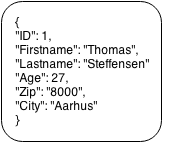
\includegraphics[scale=0.8]{Document.png} 
%% 	\captionsetup{format=plain,font=footnotesize,labelfont={bf,defaultCapFont},labelsep=quad,singlelinecheck=no}
%% 	\caption[Document store]{
%% 		\label{fig:DocumentStore}
%% 		\footnotesize{%
%% 			Document store structure.
%% 		} 
%% 	}
%% \end{figure}
%
%\subsubsection{Key-value stores}
%The key-value stores can be compared to a hashmap since every entry has a key and an associated value. 
%To retrieve data you search for the key. 
%The values can contain any kind of data from simple text to lists or documents.
%
%Primary use includes fast lookup for instance for user sessions or product lists.
%
%\begin{figure}
%	\centering
%
%	\begin{tikzpicture} [
%			diagram item/.style={
%				minimum width=3cm,
%				minimum height=1cm,
%				draw,
%				rectangle
%			}
%		]
%		\node[diagram item] (a) {Key: User1};
%		\node[diagram item, right=.5cm of a] (b) {Value: Stefan};
%
%		\node[diagram item, below=.2cm of a] (c) {Key: User2};
%		\node[diagram item, right=.5cm of c] (d) {Value: Thomas};
%
%	    \draw[arrows=->] (a) to (b);
%	    \draw[arrows=->] (c) to (d);
%	\end{tikzpicture}
%
%	\captionsetup{format=plain,font=footnotesize,labelfont={bf,defaultCapFont},labelsep=quad,singlelinecheck=no}
%		\caption[Key-value store]{
%			\label{fig:KeyValueStore}
%			\footnotesize{%
%				Key-value store structure.
%			} 
%		}
%\end{figure}
%
%% \begin{figure}
%% 	\centering
%% 	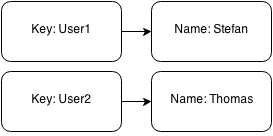
\includegraphics[scale=0.8]{KeyValue.png} 
%% 	\captionsetup{format=plain,font=footnotesize,labelfont={bf,defaultCapFont},labelsep=quad,singlelinecheck=no}
%% 	\caption[Key-value store]{
%% 		\label{fig:KeyValueStore}
%% 		\footnotesize{%
%% 			Key-value store structure.
%% 		} 
%% 	}
%% \end{figure}
%
%\subsubsection{Column-family stores}
%Column-family stores keep related data stored together.
%A column-family object consists of a key-value pair where the value contains columns of related data.
%
%Primary use includes distributed data storage, batch processing of data and analytical processing for statistical use.
%
%\begin{figure}
%	\centering
%
%	\begin{tikzpicture} [
%			diagram item/.style={
%				minimum width=3cm,
%				minimum height=1cm,
%				draw,
%				rectangle
%			},
%			diagram bigitem/.style={
%				minimum width=3cm,
%				minimum height=2cm,
%				draw,
%				rectangle
%			}
%		]
%
%
%		\node (a) {Row key};
%		\node [right=5.7cm of a] (b) {Columns};
%		\node[diagram bigitem, below=0cm of a] (c) {User1};
%		
%		%Attribute names
%		\node[diagram item, right=1.5cm of c, anchor=south] (d) {Firstname};
%		\node[diagram item, right=0cm of d] (e) {Lastname};
%		\node[diagram item, right=0cm of e] (f) {Age};
%		\node[diagram item, right=0cm of f] (g) {Zip};
%
%		%Attribute values
%		\node[diagram item, below=0cm of d] (h) {Thomas};
%		\node[diagram item, below=0cm of e] (i) {Steffensen};
%		\node[diagram item, below=0cm of f] (j) {27};
%		\node[diagram item, below=0cm of g] (k) {8000};
%
%		\node[diagram bigitem, below=.2cm of c] (l) {User2};
%		
%		%Attribute names
%		\node[diagram item, right=1.5cm of l, anchor=south] (m) {Firstname};
%		\node[diagram item, right=0cm of m] (n) {Zip};
%
%		%Attribute values
%		\node[diagram item, below=0cm of m] (o) {Thomas};
%		\node[diagram item, below=0cm of n] (p) {8000};
%	\end{tikzpicture}
%
%	\caption[Column-family store]{
%		\label{fig:ColumnFamilyStore}
%		\footnotesize{%
%			Column-family store structure.
%		} 
%	}
%\end{figure}
%
%% \begin{figure}
%% 	\centering
%% 	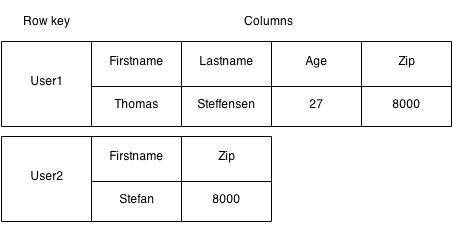
\includegraphics[scale=0.8]{ColumnFamily.png} 
%% 	\captionsetup{format=plain,font=footnotesize,labelfont={bf,defaultCapFont},labelsep=quad,singlelinecheck=no}
%% 	\caption[Column-family store]{
%% 		\label{fig:ColumnFamilyStore}
%% 		\footnotesize{%
%% 			Column-family store structure.
%% 		} 
%% 	}
%% \end{figure}
%
%\subsubsection{Graph databases}
%Graph databases divides data according to nodes and relations between nodes.
%Each node in the graph contains key-value pairs of data, and each edge describes a relationship to another node.
%Graph databases are optimized for traversal of relationships between nodes, not for data aggregation or analysis.
%
%Primary use includes pattern detection and mapping of networks.
%
%\begin{figure}
%	\centering
%	\begin{tikzpicture} [
%			diagram item/.style={
%				minimum width=5.3cm,
%				minimum height=1.5cm,
%				draw,
%				rectangle
%			}
%		]
%
%		\node[diagram item] (a) {
%			\begin{tabular}{rl}
%				Firstname:&Thomas \\
%				Lastname:&Steffensen
%			\end{tabular}};
%
%		\node[diagram item, right=3 of a] (b) {
%			\begin{tabular}{rl}
%				Firstname:&Stefan \\
%				Age:&27
%			\end{tabular}};
%
%		\node[diagram item, below=3 of a] (c) {
%			\begin{tabular}{rl}
%				Firstname:&Mette \\
%				Occupation:&Student
%			\end{tabular}};
%
%		\node[diagram item, right=3 of c] (d) {
%			\begin{tabular}{rl}
%				Name:&Aarhus Universitet
%			\end{tabular}};
%
%		\path (a) -- node[sloped] (knows) {knows} (b);
%		\path (a) -- node[sloped] (married) {married to} (c);
%		\path (a) -- node[sloped] (studies1) {studies at} (d);
%		\path (b) -- node[sloped] (studies2) {studies at} (d);
%
%	    \draw[->] (a)--(knows)--(b);
%	    \draw[->] (a)--(married)--(c);
%	    \draw[->] (a)--(studies1)--(d);
%	    \draw[->] (b)--(studies2)--(d);
%	\end{tikzpicture}
%\end{figure}
%
%% \begin{figure}
%% 	\centering
%% 	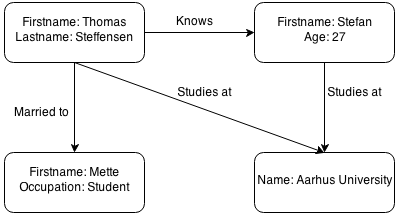
\includegraphics[scale=0.8]{Graph.png} 
%% 	\captionsetup{format=plain,font=footnotesize,labelfont={bf,defaultCapFont},labelsep=quad,singlelinecheck=no}
%% 	\caption[Graph store]{
%% 		\label{fig:GraphStore}
%% 		\footnotesize{%
%% 			Graph store structure.
%% 		} 
%% 	}
%% \end{figure}

\subsection{Relational storage that scale, NewSQL}
\label{sec:newsql}
NewSQL data stores aim to bring the relational data model into the world of horizontal scalability and flexible data models while maintaining the ACID properties and transactions of the traditional RDBMS~\cite{Cattell:ScalableSQLAndNoSQLDataStores}.
This is obtained by implementing a completely new architecture~\cite{CORBETT:SpannerGooglesGloballyDistributedDatabase}.
Starting from nothing with a new architecture allows the NewSQL data stores to be designed to take advantage of the distributed paradigms and to incorporate more flexibility into the schema structure.
The key differences between traditional SQL data stores and the NewSQL data stores are therefore found in the way the NewSQL data stores are built for scalability and throughput.
They try to avoid the major performance barriers which are locking, write-ahead logging, buffer pool overhead and latching~\cite{Stonebraker:NewSQLvsNoSQLForNewOLTP}.

Locking can be avoided by performing transactions in timestamp order or using multi version concurrency control.
Write-ahead logging can be avoided by doing automatic replication and failover.
To avoid buffer pool overhead the NewSQL data stores can run in main memory, either entirely or have a hot store in memory for active data and a cold store on disk for stale data.
To avoid latching transactions can be run single-threaded, meaning transactions must run to completion without descheduling.

Using some or all of these upgrades the NewSQL data stores can achieve higher throughput than the traditional SQL data stores.
Other features like distributed concurrency control and distributed query processing allows the NewSQL data stores to scale horizontally.

NewSQL data stores are divided into three categories~\cite{Prasanns:NewSQLTheNewWayToHandleBigData}:

\begin{itemize}
\item New databases: Completely new systems designed for scalability and throughput.
\item New MySQL storage engine: Keep the existing MySQL interface and redesign the storage engine in order to achieve scalability.
\item Transparent clustering and sharding: Provide extra features for transparent clustering and sharding on top of existing database systems. 
\end{itemize}

\subsection{SQL, NoSQL or NewSQL?}
This thesis aims to create a decentralized system with scalability and redundancy as the most important parameters.
This means that traditional SQL is not an option because of the poor scalability.

NoSQL and NewSQL has clear advantages because they are built as a consequence of the shortcomings of the traditional database systems when it comes to decentralized systems.
NoSQL has the advantage of high scalability and high throughput on data analysis, but the cost is a lack of ACID and transactions.
NewSQL promises to keep the ACID properties and transactions of the traditional database systems while simultaneously allowing horizontal scalability and high throughput.

Since both NoSQL and NewSQL seems like fitting technologies for data management in the Siemens case a further comparison between two state of the art implementations must be done in order to decide which technology will be the best suited.

\subsection{State of the art NoSQL}
To identify state of the NoSQL and NewSQL databases a website called  \inlineURL{db-engines.com}~\cite{db-engines} is used.
This website maintain a list of more than 200 different databases ranked by popularity. The list is updated monthly based on search engine popularity, discussion threads, job-offers, mentions on LinkedIn and tweets. This does not give the complete and objective ranking but it gives a pointer to the most popular database in their respective category.

Since we expect a stream of measured values from a wide range of parameters on every turbine a key-value store seems to be the obvious choice of NoSQL storage method. On top of the continuous stream of measured values aggregated measures must be obtained for the entire farm. This implies that custom software must be built to aggregate data from all the data stores and calculate aggregated values or that the data store has built in features for aggregation and calculation of aggregate values. Furthermore it is important that the database management system is able to do replication of data and automatic failover in order to achieve high availability.
Within the top 20 databases on the list we find 5 NoSQL databases:

\begin{itemize}
\item MongoDB~\cite{mongodb} ranked 5.
\item Cassandra~\cite{cassandra} ranked 9.
\item Redis~\cite{redis} ranked 12.
\item HBase~\cite{hbase} ranked 15.
\item Memcached~\cite{memcached} ranked 18.
\end{itemize}

Redis and Memcached are both key-value stores. Memcached is a very simply yet powerful distributed memory caching system.
It operates with a key for every entry and a value of raw data.
Memcached does not understand data structures so data must be serialized before upload.
Memcache does not support replication neither does it support advanced aggregate operations.

Redis is a more advanced key-value store.
It allows storing of data structures like lists, sets, hashmaps and so on.
Redis does not support aggregate operations.
Redis does not itself allow sharding but an extension called Redis Cluster do. This extension has just entered beta test phase and is not yet production ready.

Since both the key-value stores in the top 20 databases are used more like distributed memory than data stores they maintain a very simplistic approach to the interaction with data.
None of them support aggregate operations which is crucial for doing calculation over the entire farm.

The remaining NoSQL data stores are either document stores, MongoDB, or column-family stores, Cassandra and HBase.
Since data mostly has the structure of a parameter and a value it seems excessive to use a column-family data store. 
Column-family data stores are used for columns of related data which is sparse in this system.

That leaves the document store. MongoDB uses JSON-style documents to store data.
It can replicate and shard data. 
There is support for automatic failover if an instance is unavailable.
MongoDB supports data aggregation and mapreduce allowing aggregate operations before data is returned from the database.
In terms of availability, data distribution and aggregate operations MongoDB is the best of the NoSQL data stores.

\subsection{State of the art NewSQL}
Looking at the db-engines.com database list once more we find that the four highest ranking NewSQL databases are within the top 100 databases:

\begin{itemize}
\item SAP HANA~\cite{saphana} ranked 23.
\item Drizzle~\cite{drizzle} ranked 74.
\item NouDB~\cite{nuodb} ranked 83.
\item VoltDB~\cite{voltdb} ranked 90.
\end{itemize}

SAP HANA is developed by SAP.
It combines database and data processing in-memory.
SAP HANA supports planning, text processing and business analytics.
The platform has a lot of features but it is too excessive for this system.

Drizzle is an open source fork of MySQL reimplemented to support a plugin-based architecture.
The reimplementation is mainly focused on optimization for cloud infrastructure and web applications.
Lately it seems that the development has slowed and the project stalled.
The project homepage have several dead links and the last modification to the code was in may 2014.

NuoDB is a peer-to-peer oriented approach to the scalable database. Certain processes called Transaction Managers and Storage Managers share data on a peer-to-peer basis with no single point of failure.
This architecture supports sharding and replication.
What further separates NuoDB from the other NewSQL data stores is its ease of configuration and deployment. When a new instance is started it will automatically start communication with its peers. Administration of the database is done through a simple interface or administration can be set to run automatic.

VoltDB is a database built with the limitations of the traditional database systems in mind. Its focus is to avoid these limitations to achieve high throughput and scalability. The database is promoted on its high throughput compared to both traditional SQL databases and to other NoSQL and NewSQL databases.

Since all NewSQL databases are built for scalability, availability and use SQL as the query language they are able to scale, replicate and aggregate data.
In terms of ease of use NuoDB is the best choice but in terms of throughput VoltDB has some impressive benchmarks.
Since this system is a production system with feedback loops lasting only milliseconds throughput is important and that is why VoltDB is the best NewSQL alternative.

\subsection{Comparison of MongoDB and VoltDB}
Since MongoDB and VoltDB are the best fit to the Siemens Case in their respective categories a comparison of the two will determine which to use.
The comparison is based on the parameters presented in \cref{sec:databaseStorage}.
\begin{table}
	\begin{tabular}{l >{\centering}m{5cm} c}
		\hline
		\hline
		\textbf{Parameters} & \textbf{MongoDB} & \textbf{VoltDB} \\
		\hline
		\hline
		Scalability & \checkmark & \checkmark \\
		\hline
		Availability & \checkmark & \checkmark \\
		\hline
		Replication & \checkmark & \checkmark \\
		\hline
		Failover & \checkmark & \checkmark \\
		\hline
		Sharding & \checkmark & \checkmark \\
		\hline
		Aggregation & \checkmark & \checkmark \\
		\hline
		\hline
		\textbf{Additional parameters} & &\\
		\hline
		\hline
		Query language & JSON & SQL \\
		\hline
		Flexible schema & \checkmark & \text{x}  \\
		\hline
		Transactions & \text{x} & \checkmark  \\
		\hline
		ACID & \text{x} & \checkmark  \\
		\hline
		Industrial solutions & Orange, Forbes, Cisco, eBay, IBM, Microsoft, The Guardian & Schneider Electronics, Openet \\
		\hline
		\hline
	\end{tabular}
	
	\caption[MongoDB VoltDB]{
		\label{tab:mongovolt}
		\footnotesize{%
			Comparison of MongoDB and VoltDB.
		} 
	}
\end{table}

\subsection{Conclusion}
Choosing a data store these days is not easy. The data store business has been the disrupted by the amount of data generated by web 2.0. 
A number of new databases has spawned trying to solve the problems of traditional RDBMSs. 
The industry has not yet come to terms with the correct solution to the big data problem and therefore the best fitting solution as of now must be found.
MongoDB and VoltDB are two very different approaches to solve one problem.
MongoDB provides a tested solution that is very popular. VoltDB is the new solution promising even better features than MongoDB but the adaptation is still narrow.
For the Siemens case we choose MongoDB as the database.
The wider industry adaptation is a clear sign that MongoDB is a more mature and stable solution.
The popularity of MongoDB also means that a lot of resources and help is available.
MongoDB is a proven solution compared to the promising but yet untested VoltDB.